\usetikzlibrary{trees}
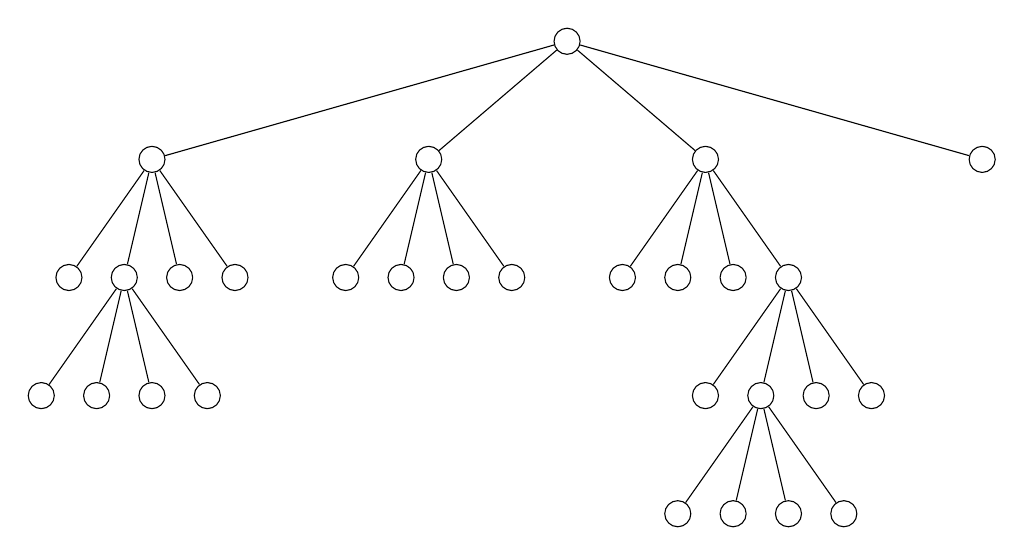
\begin{tikzpicture}[level 1/.style = {sibling distance=10em},   % <-- added
level 2/.style = {sibling distance=2em},    % <-- added
level 3/.style = {sibling distance=2em}]
\node[circle,draw](z){}{
  	child{node[circle,draw]{} 
		child{node[circle,draw]{}} 
		child {node[circle,draw]{} 
			child{node[circle,draw]{}}
			child{node[circle,draw]{}}
			child{node[circle,draw]{}}
			child{node[circle,draw]{}}
			}
		child {node[circle,draw]{}}
		child {node[circle,draw]{}}
		}
	child{node[circle,draw]{} 
			child{node[circle,draw]{}}
			child{node[circle,draw]{}}
			child{node[circle,draw]{}}
			child{node[circle,draw]{}}
			}
	child{node[circle,draw]{} 
		child{node[circle,draw]{}} 
		child {node[circle,draw]{}}
		child {node[circle,draw]{}}
		child {node[circle,draw]{} 
			child{node[circle,draw]{}}
			child{node[circle,draw]{} 
				child{node[circle,draw]{}}
				child{node[circle,draw]{}}
				child{node[circle,draw]{}}
				child{node[circle,draw]{}}
				}
			child{node[circle,draw]{}}
			child{node[circle,draw]{}}
			}
		}
  	child{node[circle,draw]{} {child[missing]}}
	};
\end{tikzpicture}